\documentclass[11pt,a4paper]{article}

\usepackage[margin=1.8cm]{geometry}
\usepackage[T1]{fontenc}
\usepackage[utf8]{inputenc}
\usepackage{lmodern}
\usepackage{microtype}
\usepackage{xcolor}
\usepackage{tikz}
\usepackage{hyperref}
\usetikzlibrary{arrows.meta,positioning,shapes.geometric}

\definecolor{navy}{HTML}{17365D}
\definecolor{softblue}{HTML}{EAF2F8}
\definecolor{softgreen}{HTML}{EAF7EF}
\definecolor{softgray}{HTML}{F4F6F7}
\definecolor{accent}{HTML}{9C640C}

\hypersetup{
  colorlinks=true,
  linkcolor=navy,
  urlcolor=navy,
  pdftitle={Pipeline Overview for Monthly Stock Return Prediction},
  pdfauthor={Momen Ismail}
}

\pagestyle{empty}

\tikzset{
  box/.style={
    rectangle,
    rounded corners=3pt,
    draw=navy,
    fill=softblue,
    very thick,
    text width=4.7cm,
    minimum height=1.2cm,
    align=center,
    font=\small
  },
  data/.style={
    rectangle,
    rounded corners=3pt,
    draw=accent,
    fill=softgreen,
    very thick,
    text width=4.7cm,
    minimum height=1.1cm,
    align=center,
    font=\small
  },
  output/.style={
    rectangle,
    rounded corners=3pt,
    draw=black!55,
    fill=softgray,
    very thick,
    text width=4.7cm,
    minimum height=1.1cm,
    align=center,
    font=\small
  },
  arrow/.style={-{Latex[length=3mm]}, very thick, draw=navy}
}

\begin{document}

\begin{center}
{\LARGE\bfseries\color{navy} Pipeline Overview}\\[0.2cm]
{\large Monthly Stock Return Prediction Data Construction}\\[0.4cm]
{\small Final model sample: January 1990--December 2025}
\end{center}

\vspace{0.3cm}

\begin{center}
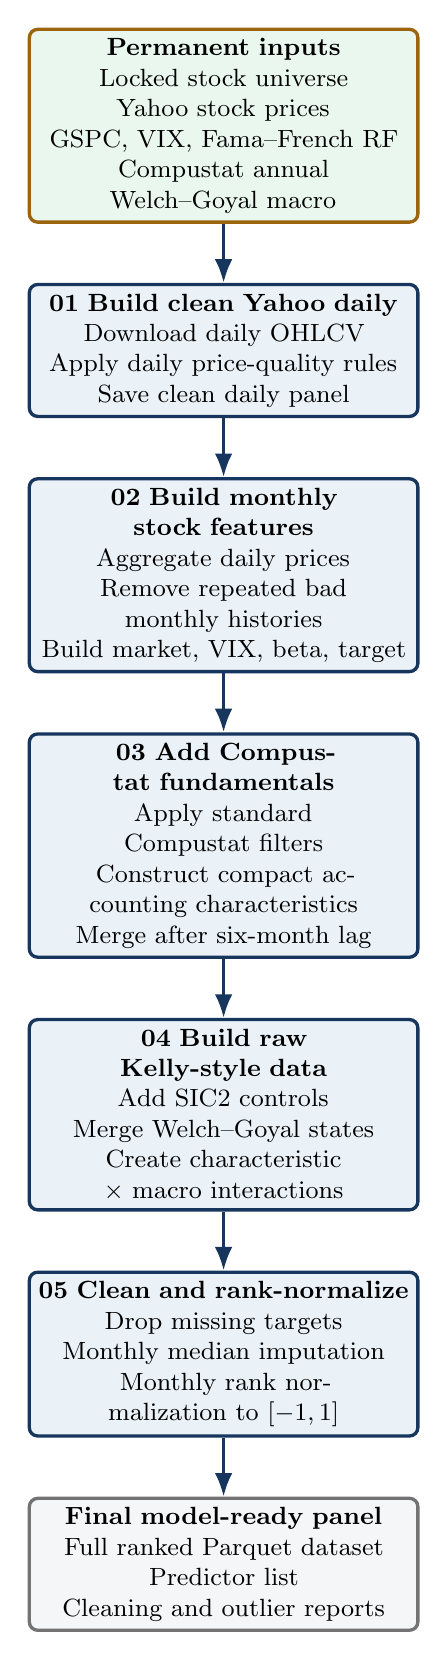
\begin{tikzpicture}[node distance=0.75cm and 1.2cm]

\node[data] (inputs) {
\textbf{Permanent inputs}\\
Locked stock universe\\
Yahoo stock prices\\
GSPC, VIX, Fama--French RF\\
Compustat annual\\
Welch--Goyal macro
};

\node[box, below=of inputs] (s01) {
\textbf{01 Build clean Yahoo daily}\\
Download daily OHLCV\\
Apply daily price-quality rules\\
Save clean daily panel
};

\node[box, below=of s01] (s02) {
\textbf{02 Build monthly stock features}\\
Aggregate daily prices\\
Remove repeated bad monthly histories\\
Build market, VIX, beta, target
};

\node[box, below=of s02] (s03) {
\textbf{03 Add Compustat fundamentals}\\
Apply standard Compustat filters\\
Construct compact accounting characteristics\\
Merge after six-month lag
};

\node[box, below=of s03] (s04) {
\textbf{04 Build raw Kelly-style data}\\
Add SIC2 controls\\
Merge Welch--Goyal states\\
Create characteristic $\times$ macro interactions
};

\node[box, below=of s04] (s05) {
\textbf{05 Clean and rank-normalize}\\
Drop missing targets\\
Monthly median imputation\\
Monthly rank normalization to $[-1,1]$
};

\node[output, below=of s05] (final) {
\textbf{Final model-ready panel}\\
Full ranked Parquet dataset\\
Predictor list\\
Cleaning and outlier reports
};

\draw[arrow] (inputs) -- (s01);
\draw[arrow] (s01) -- (s02);
\draw[arrow] (s02) -- (s03);
\draw[arrow] (s03) -- (s04);
\draw[arrow] (s04) -- (s05);
\draw[arrow] (s05) -- (final);

\end{tikzpicture}
\end{center}

\newpage

\begin{center}
{\Large\bfseries\color{navy} Timing and Leakage Controls}
\end{center}

\vspace{0.4cm}

\begin{center}
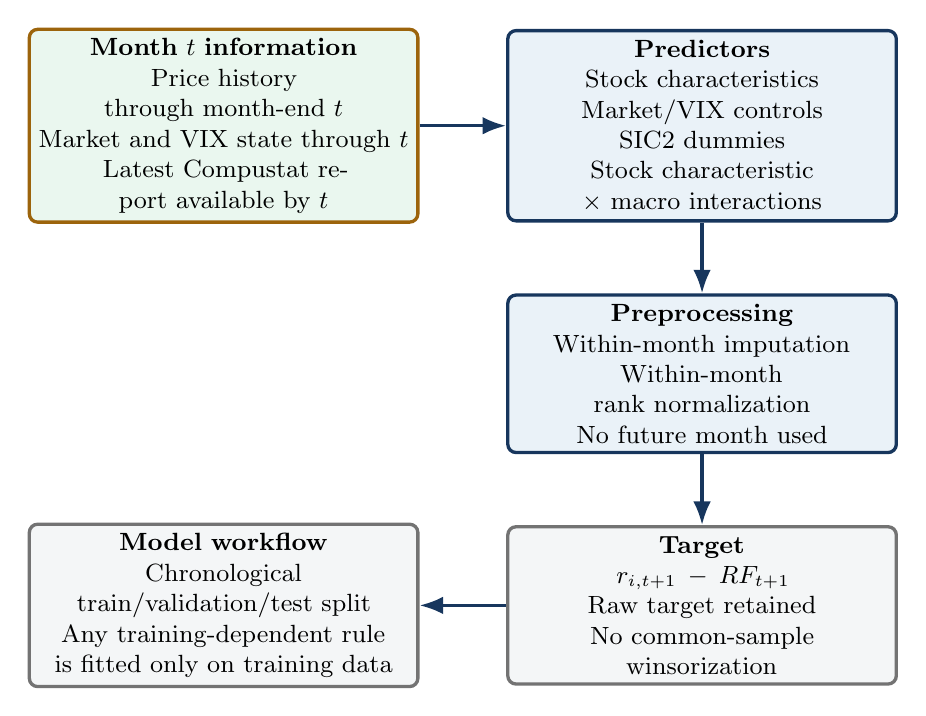
\begin{tikzpicture}[node distance=0.9cm and 1.1cm]

\node[data] (montht) {
\textbf{Month $t$ information}\\
Price history through month-end $t$\\
Market and VIX state through $t$\\
Latest Compustat report available by $t$
};

\node[box, right=of montht] (predictors) {
\textbf{Predictors}\\
Stock characteristics\\
Market/VIX controls\\
SIC2 dummies\\
Stock characteristic $\times$ macro interactions
};

\node[box, below=of predictors] (preprocess) {
\textbf{Preprocessing}\\
Within-month imputation\\
Within-month rank normalization\\
No future month used
};

\node[output, below=of preprocess] (target) {
\textbf{Target}\\
$r_{i,t+1}-RF_{t+1}$\\
Raw target retained\\
No common-sample winsorization
};

\node[output, left=of target] (models) {
\textbf{Model workflow}\\
Chronological train/validation/test split\\
Any training-dependent rule is fitted only on training data
};

\draw[arrow] (montht) -- (predictors);
\draw[arrow] (predictors) -- (preprocess);
\draw[arrow] (preprocess) -- (target);
\draw[arrow] (target) -- (models);

\end{tikzpicture}
\end{center}

\vspace{0.4cm}

\begin{center}
\begin{tabular}{p{4.2cm}p{10.2cm}}
\textbf{Accounting timing} & Annual Compustat data are available only after a six-month reporting lag and are merged backward into each stock-month.\\[0.2cm]
\textbf{Target timing} & A row dated month $t$ predicts next-month excess return, $r_{i,t+1}-RF_{t+1}$.\\[0.2cm]
\textbf{Cross-sectional preprocessing} & Imputation and rank normalization use only firms observed in the same month.\\[0.2cm]
\textbf{Sample endpoint} & January 2026 prices may realize the December 2025 target, but final rows end at December 2025.\\
\end{tabular}
\end{center}

\end{document}
